
%(BEGIN_QUESTION)
% Copyright 2015, Tony R. Kuphaldt, released under the Creative Commons Attribution License (v 1.0)
% This means you may do almost anything with this work of mine, so long as you give me proper credit

\noindent
{\bf Lab Exercise -- introduction}

\vskip 5pt

Your task is to build, document, and troubleshoot a {\it split range} valve system with another team, where a pair of control valves are controlled from the control room area by adjusting the output of a single ``Hand Indicating Controller'' (HIC) in its ``manual'' mode.  Each control valve will use a positioner to implement the split-ranges.  Each instrument in the loop should be labeled with a proper tag name (e.g. ``HV-78a'' and ``HV-78b'' for two split-ranged, hand-controlled valves), with all instruments in each loop sharing the same loop number.  Write on pieces of masking tape to make simple labels for all the instruments and signal lines.

The following table of objectives show what you and your team must complete within the scheduled time for this lab exercise.  Note how some of these objectives are individual, while others are for the team as a whole:

\underbar{Objective completion table:}

% No blank lines allowed between lines of an \halign structure!
% I use comments (%) instead, so that TeX doesn't choke.

$$\vbox{\offinterlineskip
\halign{\strut
\vrule \quad\hfil # \ \hfil & 
\vrule \quad\hfil # \ \hfil & 
\vrule \quad\hfil # \ \hfil & 
\vrule \quad\hfil # \ \hfil & 
\vrule \quad\hfil # \ \hfil & 
\vrule \quad\hfil # \ \hfil & 
\vrule \quad\hfil # \ \hfil \vrule \cr
\noalign{\hrule}
%
% First row
{\bf Performance objective} & {\bf Grading} & {\bf 1} & {\bf 2} & {\bf 3} & {\bf 4} & {\bf Team} \cr
%
\noalign{\hrule}
%
% Another row
Prototype sketch ({\it before building the system!}) & mastery & -- & -- & -- & -- & \cr
%
\noalign{\hrule}
%
% Another row
Final loop diagram and system inspection & mastery & & & & & -- -- -- -- \cr
%
\noalign{\hrule}
%
% Another row
Split-range calibration (with saturation) & mastery & -- & -- & -- & -- &  \cr
%
\noalign{\hrule}
%
% Another row
Demonstration of working system & mastery & -- & -- & -- & -- & \cr
%
\noalign{\hrule}
%
% Another row
Troubleshooting & mastery & & & & & -- -- -- -- \cr
%
\noalign{\hrule}
%
% Another row
Lab question: Selection/testing & proportional &  &  &  &  & -- -- -- -- \cr
%
\noalign{\hrule}
%
% Another row
Lab question: Commissioning & proportional &  &  &  &  & -- -- -- -- \cr
%
\noalign{\hrule}
%
% Another row
Lab question: Mental math & proportional &  &  &  &  & -- -- -- -- \cr
%
\noalign{\hrule}
%
% Another row
Lab question: Diagnostics & proportional &  &  &  &  & -- -- -- -- \cr
%
\noalign{\hrule}
%
% Another row
Decommission and lab clean-up & mastery & -- & -- & -- & -- &  \cr
%
\noalign{\hrule}
} % End of \halign 
}$$ % End of \vbox

The only ``proportional'' scoring in this activity are the lab questions, which are answered by each student individually.  A listing of potential lab questions are shown at the end of this worksheet question.  The lab questions are intended to guide your labwork as much as they are intended to measure your comprehension, and as such the instructor may ask these questions of your team day by day, rather than all at once (on a single day).

%\vskip 10pt

{\bf It is essential that your team plans ahead what to accomplish each day.  A short (10 minute) team meeting at the beginning of each lab session is a good way to do this, reviewing what's already been done, what's left to do, and what assessments you should be ready for.  There is a lot of work involved with building, documenting, and troubleshooting these working instrument systems!}

As you and your team work on this system, you will invariably encounter problems.  You should always attempt to solve these problems as a team before requesting instructor assistance.  If you still require instructor assistance, write your team's color on the lab whiteboard with a brief description of what you need help on.  The instructor will meet with each team in order they appear on the whiteboard to address these problems.

$$\includegraphics[width=15.5cm]{i00787x01.eps}$$

\vfil \eject

\noindent
{\bf Lab Exercise -- installing a positioner on the valve}

\vskip 5pt

You team will need to install a positioner on the control valve you formerly ``rebuilt'' to facilitate split-ranging.  While valves lacking positioners can be split-ranged, the task of split-ranging is greatly simplified by using a positioner because it is relatively easy to change zero and span settings.  It is recommended that your team coordinate with one other team in order to build a split-range valve pair, and that you use different models of positioner.

An important first step should be finding appropriate documentation for your valve positioner.  Nearly every instrument in the lab is documented electronically at the manufacturer's website, so your best resource is the Internet (and/or your Instrumentation Reference where a variety of instrument manuals have been downloaded for you).  Use this documentation to identify how to properly install, wire, tube, and calibrate the positioner.  Your instructor will check to see you have located and are familiar with the equipment manual(s).

The control valve should have mounting holes on its actuator assembly for receiving a positioner bracket.  This metal bracket will serve as the mounting ``platform'' for the positioner once attached to the valve actuator.  Brackets and positioners are not universal in design -- that is, they are made to match each other.

\vskip 10pt

{\bf A detail important for both safety and time management is to make sure you do not disturb the coupling of the valve body and actuator stems when connecting the positioner to the stem.}  On Fisher sliding-stem valves, particularly, the stem connector bolts must be un-done to attach the positioner's feedback linkage.  If the stem connector is loosened with full spring force applied to the valve seat (as is the case with any sliding-stem, air-to-open valve when no air pressure is applied), the actuator stem will slip loose and suddenly shift.  This will not only hurt your fingers if they are in the way of the actuator stem when it slips, but it will also necessitate a re-setting of the coupling between the valve body and actuator stems which can be time-consuming.

{\bf To avoid this problem on air-to-open valves, first apply enough air pressure to the actuator to raise the plug off the seat and relieve the seating force before loosening the stem coupling!}  With the valve plug held off the seat by air pressure, you may loosen the stem coupling with no risk of harm to yourself and little risk of disturbing the coupling position.

Another important detail regarding positioner installation is properly aligning the linkage between the positioner and the control valve stem.  Improper linkage alignment will result in non-linear valve travel (i.e. if 0\% and 100\% is accurate, 25\%, 50\% and/or 75\% will not be).  Again, consult the manufacturer's documentation for instructions on how to properly align the positioner-to-stem linkage.

\vskip 10pt

Positioners act as ``position controllers'' for control valves, sending enough air pressure as necessary to move the valve to match the signal given by the controller's output.  As controllers in their own right, positioners require a supply of compressed air to ``power'' them.  This air supply often needs to be of a different (greater) pressure than the air supply of an I/P signal converter.  For piston-actuated valves, the positioner often runs on 100 PSI compressed air, while the I/P converter runs on only 20 PSI.  As always, consult the manufacturer's manual for air supply specifications.

\vskip 10pt

{\bf Common mistakes:}

\begin{itemize}
\item{} Not checking valve stroke length for proper configuration before installing the positioner.
\item{} Disturbing the valve body/actuator stem coupling by disassembling the coupling when the actuator spring pressure is still seating the plug.
\item{} Incorrect installation and/or alignment of the linkage coupling the positioner to the valve stem: {\it consult the manual when installing your team's positioner to see exactly how it should attach!}
\item{} Improper pipe/tube fitting installation (e.g. trying to thread tube fittings into pipe fittings and vice-versa).
\end{itemize}




\vfil \eject

\noindent
{\bf Lab Exercise -- calibrating the positioner}

\vskip 5pt

When finished installing the positioner, you should test it prior to building the rest of the loop system.  Simply simulate the output signal of a loop controller by using a 4-20 mA loop calibrator in ``source'' mode, driving a signal to the I/P (or to the positioner directly, depending on the model) to stroke the valve.  

$$\includegraphics[width=15.5cm]{i00787x02.eps}$$

One of the criteria for a successful positioner calibration is that the positioner must ``saturate'' its output pressure(s) when the valve reaches full stroke.  For example, on a simple air-to-open valve calibration (i.e. 4 mA = valve at 0\% position ; 20 mA = valve at 100\% position), the positioner should saturate at beyond bench-set pressure at full signal (20 mA) and saturate at 0 PSI at minimum signal (4 mA) to ensure full seat loading.  This requirement is in addition to accurate positioning at all points between 0\% and 100\%.

\vskip 10pt

Mechanical positioners have interactive ``zero'' and ``span'' calibration adjustments much like analog transmitters, requiring multiple adjustments to get right.  Digital ``smart'' positioners are comparatively easy to set up because they often have their own self-calibration mode where the positioner finds the valve's stroke limits automatically and calibrates itself between those limits.  In either case, you should consult the manufacturer's documentation to determine a calibration procedure for your valve's positioner.

You will need to agree with the other team on a particular split-ranging scheme (e.g.  complementary, exclusive, or progressive), then calibrate each valve accordingly:

$$\includegraphics[width=15.5cm]{i00787x03.eps}$$

Be sure to note the limitations of your team's valve when deciding on a split range: some positioners are limited in the ranges they can handle (e.g. some models of Fisher DVC6000 positioner cannot be configured for reverse action)!

\vskip 10pt

{\bf Common mistakes:}

\begin{itemize}
\item{} Calibrating the I/P converter for a non-standard range (i.e. something other than 3-15 PSI) instead of using the positioner's calibration to achieve split-ranging
\item{} Not learning about the {\it other} positioner (different model) in your split-range loop, but rather focusing exclusively on your team's positioner
\item{} Incorrect supply pressure given to positioner
\end{itemize}


\vskip 10pt

{\bf Installing and roughly calibrating a positioner should take no more than one full lab session (3 hours) if all components are readily available and the team is working efficiently!}




\vfil \eject

\noindent
{\bf Lab Exercise -- selecting components and planning the system}

\vskip 5pt

One of the most common problems students encounter when building any working system, whether it be a circuit on a solderless breadboard or an instrument loop spanning an entire room, is properly connecting and configuring all components.  An unfortunate tendency among most students is to simply start connecting parts together, essentially designing the system as they go.  This usually leads to improperly-connected components and non-functioning systems, sometimes with the result of destroying components due to those improper connections!

An alternative approach is to plan ahead by designing the system before constructing it.  This is easily done by sketching a diagram showing how all the components should interconnect, then analyzing that diagram and making changes before connecting anything together.  When done as a team, this step ensures everyone is aware of how the system should work, and how it should go together.  The resulting ``prototype'' diagram need not be complex in detail, but it should be detailed enough for anyone to see which component terminals (and ports) connect to terminals and ports of other devices in the system.  For example, your team's prototype sketch should be clear enough to determine all DC electrical components will have the correct polarities.  If your proposed system contains a significant amount of plumbing (pipes and tubes), your prototype sketch should show all those connections as well.

\vskip 10pt

Your team's prototype sketch is so important that the instructor will demand you provide this plan before any construction on your team's working system begins.  {\it Any team found constructing their system without a verified plan will be ordered to cease construction and not resume until a prototype plan has been drafted and approved!}  Each member on the team should have ready access to this plan (ideally possessing their own copy of the plan) throughout the construction process.  Prototype design sketching is a skill and a habit you should cultivate in school and take with you in your new career.

\vskip 10pt

{\bf Planning a functioning system should take no more than an hour if the team is working efficiently, and will save you hours of frustration (and possible component destruction!).}







\vfil \eject

\noindent
{\bf Lab Exercise -- building the system}

\vskip 5pt

The Instrumentation lab is set up to facilitate the construction of working instrument ``loops,'' with over a dozen junction boxes, pre-pulled signal cables, and ``racks'' set up with 2-inch vertical pipes for mounting instruments.  The only wires you should need to install to build a working system are those connecting the field instrument to the nearest junction box, and then small ``jumper'' cables connecting different pre-installed cables together within intermediate junction boxes.

After getting your prototype sketch approved by the instructor, you are cleared to begin building the split-ranged valve system.  This will consist of a loop controller placed into ``manual'' mode to allow direct control over the position of your team's valve as well as the valve of one more team.  

The teams pairing up to build a split-range valve loop should use different models of positioner so that students from each team get to work with multiple positioner models.  Even though your team is accountable for only calibrating your valve's positioner, each person on both teams should take the time to learn how the other valve's positioner is calibrated.  If one positioner is all-mechanical and the other is ``smart,'' the differences will be dramatic!

There will be no transmitter installed in this loop.  Feel free to use 1/4 inch plastic tubing for all pneumatic signal connections, and be sure not to exceed the rated supply pressure for the I/P (as documented in the I/P manual).

Select a specific loop controller to act as a display indicator for your system.  Your instructor may choose the controller for your team, to ensure you learn more than one type of controller during the course of a quarter.  The controller itself should be labeled ``HC-'' or ``HIC-'' because it is a ``hand'' controller, allowing a human operator manual control over the valve's position. 

Note that for some positioners, dual 4-20 mA output signals from the controller will be necessary to connect the two valves together to form one split-range loop.  This is especially true when pairing ``smart'' positioners, which may not be able to digitally communicate if two of them are in the same 4-20 mA series circuit due to address conflicts!  Configuring a loop controller for dual 4-20 mA outputs will require some controller re-programming.  For single-loop controllers, DCS, and DDC systems, this means adding an additional ``output'' function block to the program.  For PLC controllers, this means adding an additional rung of ladder logic.

Finally, your split-range valve system needs to have a loop number, so all instruments may be properly labeled.  This loop number needs to be unique, so that another team does not label their instruments and cables the same as yours.  One way to make your loop number unique is to form a two-digit number from the equivalent resistor color-code values for your teams' colors.  For example, if you are the ``Red'' team, and the partnering team is ``Blue,'' your loop number could be ``26''.  The two valves will then be distinguished by suffix letters (e.g. HV-26a and HV-26b).

\vskip 10pt

{\bf Common mistakes:}

\begin{itemize}
\item{} Failing to tug on each and every wire where it terminates to ensure a mechanically sound connection.
\item{} Students working on portions of the system in isolation, not sharing with their teammates what they did and how.  It is important that the whole team learns all aspects of their system!
\end{itemize}

\vskip 10pt

{\bf Building a functioning system from two working valves should take no more than one full lab session (3 hours) if all components are readily available and the team is working efficiently!}





\vfil \eject

\noindent
{\bf Lab Exercise -- documenting the system}

\vskip 5pt

Each student must sketch their own {\it loop diagram} for their team's system, following proper ISA conventions.  Sample loop diagrams are shown in the next question in this worksheet.  These loop diagrams must be {\it comprehensive} and {\it detailed}, showing every wire connection, every cable, every terminal block, range points, etc.  The principle to keep in mind here is to make the loop diagram so complete and unambiguous that anyone can follow it to see what connects to what, even someone unfamiliar with industrial instrumentation.  In industry, loops are often constructed by contract personnel with limited understanding of how the system is supposed to function.  The loop diagrams they follow must be so complete that they will be able to connect everything properly without necessarily understanding how it is supposed to work.

Every instrument and every signal cable in your loop needs to be properly labeled with an ISA-standard tag number.  An easy way to do this is to wrap a short piece of masking tape around each cable (and placed on each instrument) then writing on that masking tape with a permanent marker.  Although no industry standard exists for labeling signal cables, a good recommendation is to label each two-wire cable with the tag number of the field instrument it goes to.  Thus, every length of two-wire cable in a hand valve circuit should be labeled ``HV-$x$'' (where ``$x$'' is the loop number).  If you are using two separate cables for the split-ranged valves, differentiate one from the other by using suffix letters (e.g. HV-26a and HV-26b).

When your entire team is finished drafting your individual loop diagrams, call the instructor to do an inspection of the loop.  Here, the instructor will have students take turns going through the entire loop, with the other students checking their diagrams for errors and omissions along the way.  During this time the instructor will also inspect the quality of the installation, identifying problems such as frayed wires, improperly crimped terminals, poor cable routing, missing labels, lack of wire duct covers, etc.  The team must correct all identified errors in order to receive credit for their system.  

After successfully passing the inspection, each team member needs to place their loop diagram in the diagram holder located in the middle of the lab behind the main control panel.  When it comes time to troubleshoot another team's system, this is where you will go to find a loop diagram for that system!

\vskip 10pt

{\bf Common mistakes:}

\begin{itemize}
\item{} Forgetting to label all signal wires (see example loop diagrams).
\item{} Forgetting to label all field instruments with their own tag names (e.g. PT-83).
\item{} Forgetting to note all wire colors.
\item{} Forgetting to put your name on the loop diagram!
\item{} Basing your diagram off of a team-mate's diagram, rather than closely inspecting the system for yourself.
\item{} Not placing loop sheet instruments in the correct orientation (field instruments on the left, control room instruments on the right).
\end{itemize}

\vskip 10pt

{\bf Creating and inspecting accurate loop diagrams should take no more than one full lab session (3 hours) if the team is working efficiently!}







\vfil \eject

\noindent
{\bf Lab Exercise -- troubleshooting}

\vskip 5pt

The most challenging aspect of this lab exercise is {\it troubleshooting}, where you demonstrate your ability to logically isolate a problem in the system.  All troubleshooting is done on an individual basis (no team credit!), and must be done {\it on a system you did not help build}, so that you must rely on loop diagrams to find your way around the system instead of from your own memory of building it.

Each student is given a limited amount of time to identify both the general location and nature of the fault, logically justifying all diagnostic steps taken.  All troubleshooting activities will take place under direct instructor supervision to ensure students are working independently and efficiently. 

Failure to correctly identify both the general location and nature of the fault within the allotted time, and/or failing to demonstrate rational diagnostic procedure to the supervising instructor will disqualify the effort, in which case the student must re-try with a different fault.  Multiple re-tries are permitted with no reduction in grade.

A standard multimeter is the only test equipment allowed during the time limit.  No diagnostic circuit breaks are allowed except by instructor permission, and then only after correctly explaining what trouble this could cause in a real system.  

The instructor will review each troubleshooting effort after completion, highlighting good and bad points for the purpose of learning.  Troubleshooting is a skill born of practice and failure, so do not be disappointed in yourself if you must make multiple attempts to pass!  One of the important life-lessons embedded in this activity is how to deal with failure, because it {\it will} eventually happen to you on the job!  There is no dishonor in failing to properly diagnose a fault after doing your level best.  The only dishonor is in taking shortcuts or in giving up.

\vskip 10pt

{\bf Common mistakes:}

\begin{itemize}
\item{} Neglecting to take measurements with your multimeter.
\item{} Neglecting to monitor pressure gauges on both positioners while testing the system.
\item{} Incorrectly interpreting the loop diagram (e.g. thinking you're at the wrong place in the system when taking measurements).
\item{} Incorrect multimeter usage (e.g. AC rather than DC, wrong range, wrong test lead placement).  This is especially true when a student comes to lab unprepared and must borrow someone else's meter that is different from theirs!
\end{itemize}

\vskip 10pt

{\bf Remember that the purpose of the troubleshooting exercise is to foster and assess your ability to intelligently diagnose a complex system.  Finding the fault by luck, or by trial-and-error inspection, is not a successful demonstration of skill.  The only thing that counts as competence is your demonstrated ability to logically analyze and isolate the problem, correctly explaining all your steps!}

\vskip 10pt

{\bf Troubleshooting takes a lot of lab time, usually at least two 3-hour lab sessions for everyone in a full class to successfully pass.  Be sure your team budgets for this amount of time as you plan your work, and also be sure to take advantage of your freedom to observe others as they troubleshoot, to better learn this art.}



\vfil \eject

\noindent
{\bf Lab questions}

\vskip 5pt

\begin{itemize}
\item{} {\bf Selection and Initial Testing}
\item{} Identify and explain the purpose of using a valve positioner on a pneumatic control valve
\item{} Explain what ``progressive'' split ranging is, and give a practical example of its use
\item{} Explain what ``complementary'' split ranging is, and give a practical example of its use
\item{} Explain what ``exclusive'' split ranging is, and give a practical example of its use
\item{} Explain how to properly align the linkage connecting the positioner to the valve stem, and why this alignment is important
\end{itemize}

\filbreak

\begin{itemize}
\item{} {\bf Commissioning and Documentation}
\item{} Demonstrate how to isolate potentially hazardous energy in your system ({\it lock-out, tag-out}) and also how to safely verify the energy has been isolated prior to commencing work on the system
\item{} Demonstrate the proper use of a combination wrench (which end is preferred)
\item{} Demonstrate how to use a combination wrench to turn a nut or bolt in close quarters (where there is not enough room to swing the wrench more than 20 degrees or so)
\item{} Demonstrate how to adjust the ``zero'' adjustment of a positioner
\item{} Demonstrate how to adjust the ``span'' (travel range) adjustment of a positioner
\item{} Demonstrate the use of a loop calibrator to {\it source} current to the valve
\item{} Explain how to isolate a control valve for removal and service using manual block and bypass valves
\end{itemize}

\filbreak

\begin{itemize}
\item{} {\bf Mental math} (no calculator allowed!)
\item{} Calculate the flow coefficient (Cv) for a specific control valve given pressure drop and liquid flow rate
\item{} Calculate the liquid flow rate through a specific control valve given flow coefficient (Cv) and pressure drop
\item{} Calculate the positions of both valves in a {\it complementary} split-range pair for a controller output of $x$ percent
\item{} Calculate the positions of both valves in a {\it progressive} split-range pair for a controller output of $x$ percent
\item{} Calculate the positions of both valves in an {\it exclusive} split-range pair for a controller output of $x$ percent
\item{} Calculate force generated by a diaphragm or piston actuator given diameter and applied fluid pressure in units of PSI
\end{itemize}

\filbreak

\begin{itemize}
\item{} {\bf Diagnostics}
\item{} ``Virtual Troubleshooting'' -- referencing their system's diagram(s), students propose diagnostic tests (e.g. ask the instructor what a meter would measure when connected between specified points; ask the instructor how the system responds if test points are jumpered) while the instructor replies according to how the system would behave if it were faulted.  Students try to determine the nature and location of the fault based on the results of their own diagnostic tests.
\item{} Explain how to confirm the presence of an {\it open} in a 4-20 mA signal cable using only a voltmeter (no resistance or current measurement allowed!) 
\item{} Explain how to confirm the presence of a {\it short} in a 4-20 mA signal cable using only a voltmeter (no resistance or current measurement allowed!) 
\item{} Determine whether or not a given diagnostic test will provide useful information, given a set of symptoms exhibited by a failed system
\item{} Identify at least two plausible faults given the results of a diagnostic test and a set of symptoms exhibited by a failed system
\end{itemize}



\vfil \eject

\noindent
{\bf Lab Exercise -- decommissioning and clean-up}

\vskip 5pt

The final step of this lab exercise is to decommission your team's entire system and re-stock certain components back to their proper storage locations, the purpose of which being to prepare the lab for the next lab exercise.  Remove your system documentation (e.g. loop diagram) from the common holding area, either discarding it or keeping it for your own records.  Also, remove instrument tag labels (e.g. FT-101) from instruments and from cables.  Perform general clean-up of your lab space, disposing of all trash, placing all tools back in their proper storage locations, sweeping up bits of wire off the floor and out of junction boxes, etc.

\vskip 10pt

\indent
{\bf Leave the following components in place, mounted on the racks:}

\begin{itemize}
\item{} Large control valves and positioners
\item{} I/P transducers
\item{} Large electric motors
\item{} Large variable-frequency drive (VFD) units
\item{} Cables inside conduit interconnecting junction boxes together
\item{} Pipe and tube fittings (do not unscrew pipe threads)
\item{} Supply air pressure regulators
\end{itemize}

\vskip 10pt

\indent
{\bf Return the following components to their proper storage locations:}

\begin{itemize}
\item{} Sensing elements (e.g. thermocouples, pH probes, etc.)
\item{} Process transmitters
\item{} ``Jumper'' cables used to connect terminal blocks within a single junction box
\item{} Plastic tubing and tube fittings (disconnect compression-style tube fittings)
\item{} Power cables and extension cords
\item{} Adjustment (loading station) air pressure regulators
\end{itemize}

\vskip 10pt

Finally, you shall return any control system components to their original (factory default) configurations.  This includes controller PID settings, function block programs, input signal ranges, etc.


\underbar{file i00787}
%(END_QUESTION)





%(BEGIN_ANSWER)


%(END_ANSWER)





%(BEGIN_NOTES)

\noindent
{\bf Loop diagrams / inspections:}

I strongly recommend checking off students' loop diagrams while you inspect their loop (checking for secure wiring, proper tubing, good conduit installation, etc.) with them.  Have all team members take you on a ``tour'' of their completed loop, with each team member explaining a different portion of the loop you select while using their own loop diagram as a guide.  While a student is explaining their section of the loop, you can check the other students' loop diagrams for accuracy.  This not only saves time by consolidating the tasks of loop inspection and loop diagram verification, but it also ensures students can actually relate their loop diagrams to the loop they have built and articulate that understanding to you.

\vskip 10pt

\goodbreak

\noindent
{\bf Troubleshooting fault ideas:}

\begin{itemize}
\goodbreak
\item{} Connect instrument tubes to wrong port (construction fault)
\item{} Replace I/P restrictor with pre-faulted (plugged) unit (high output fault)
\item{} Replace I/P relay with pre-faulted unit (low or high output fault)
\item{} Turn supply air pressure down well below 15 PSI (low output fault)
\item{} Strip wire at terminal, then insert insulated wire end under terminal and tighten (open wire fault)
\item{} Cut signal cable somewhere in mid-conduit (open wire fault)
\item{} Push a thumbtack through the cable somewhere in mid-conduit (shorted wire fault)
\item{} Wire instrument cable conductors backward (construction fault)
\item{} Configure transmitter for excessive damping (slow response fault)
\item{} Configure indicator/controller for excessive damping (slow response fault)
\item{} Miscalibrate transmitter and/or indicator/controller (inaccuracy fault)
\item{} Plug tube connections using portion of foam earplug stuffed into tube fitting (slow response fault)
\item{} Reverse action of controller/positioner/transmitter (wrong response fault)
\item{} Mis-configure linear/sq.root characterization of transmitter and/or indicator/controller (nonlinearity fault)
\item{} Connect 2.2 k resistor in parallel with 4-20 mA transmitter to simulate partial short in wiring (inaccuracy fault)
\item{} Exchange 250 ohm resistor for a different resistor that looks the same but has the wrong value (inaccuracy fault) 
\item{} Unplug cable(s) inside transmitter or controller (failed instrument fault)
\item{} Give students wrong loop diagram (documentation fault)
\item{} Start students out on wrong controller (operator error)
\item{} Close valve and leave safety tag hanging on it (operator/technician error)
\end{itemize}

%INDEX% Lab exercise, split-range control valves

%(END_NOTES)


